\section{Results with alternative asimov datasets}

\begin{figure}[!h!tb]
  \begin{center}

    \subfigure[$\pt(\mathrm{H})$]{
      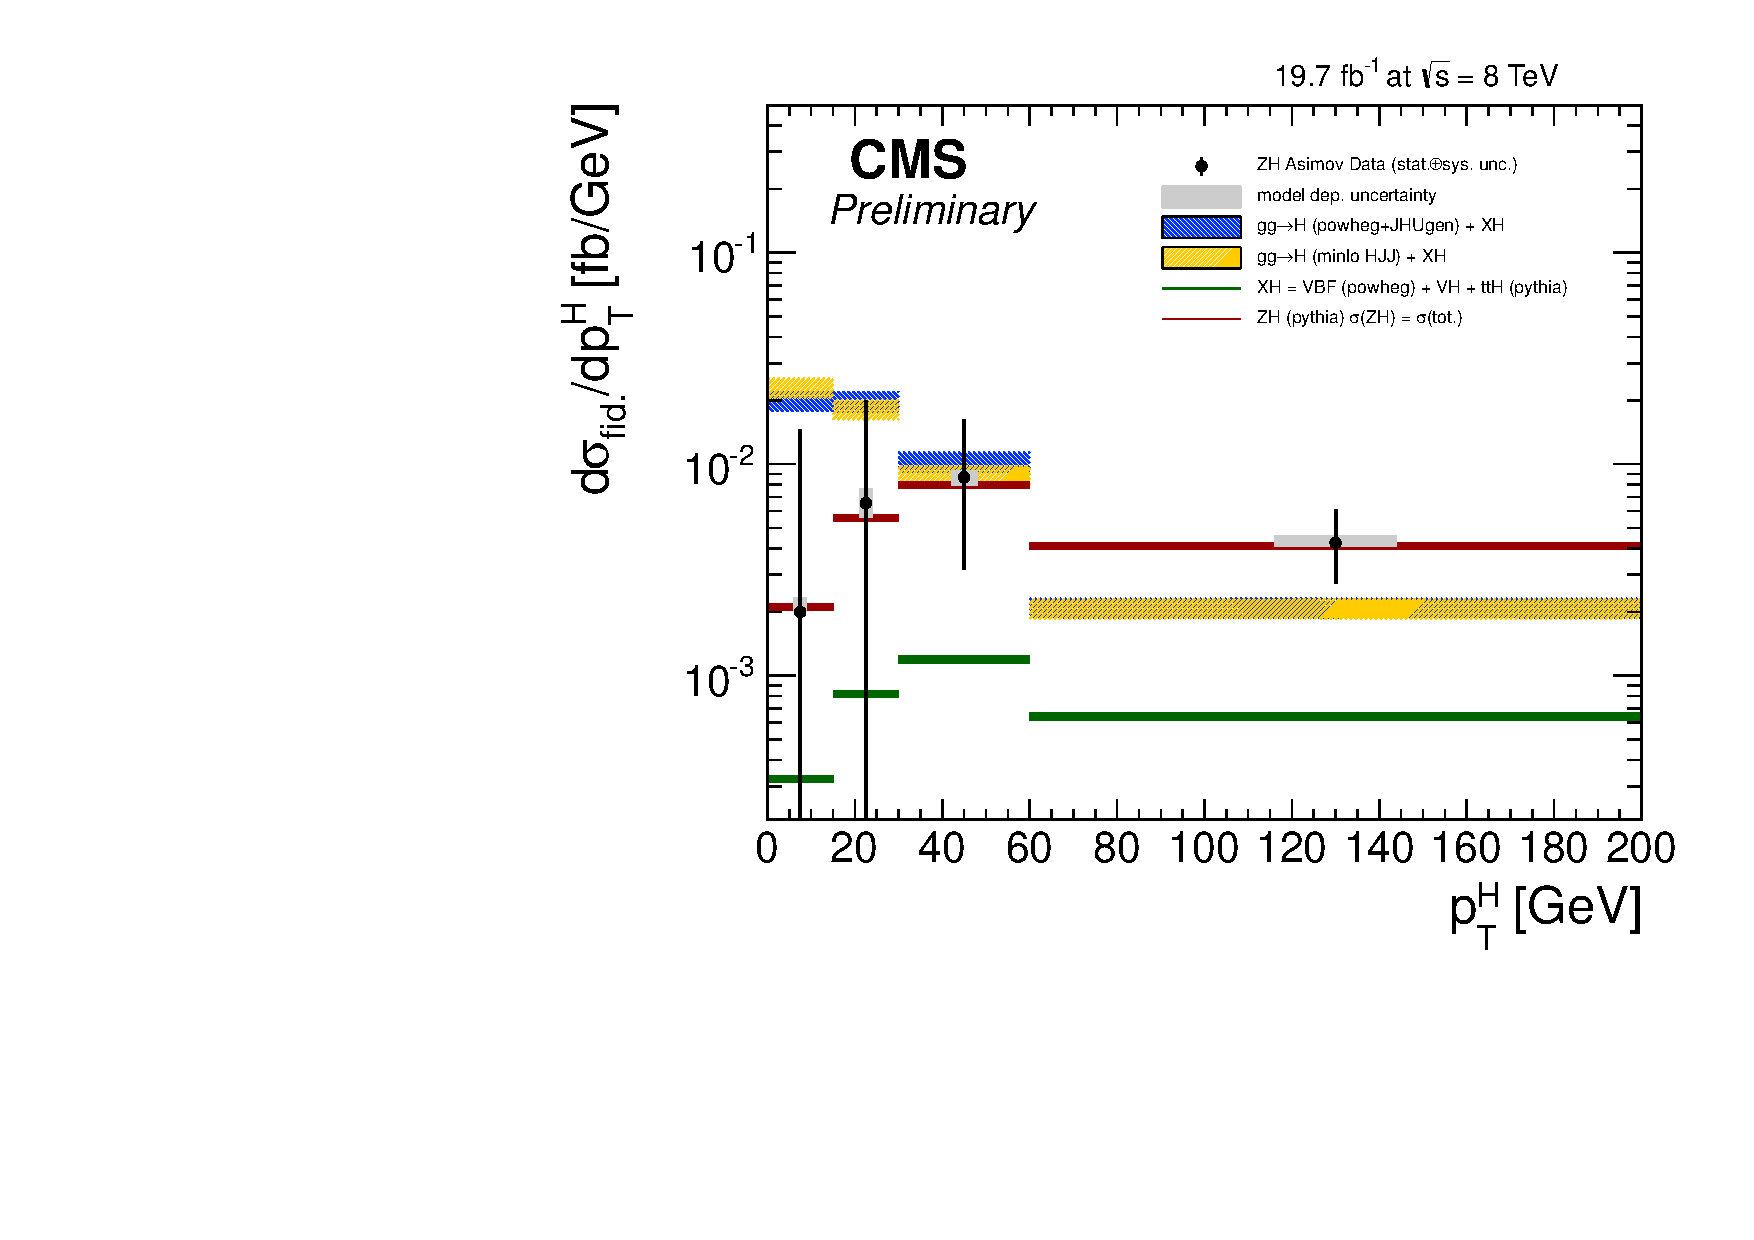
\includegraphics[width=0.48\textwidth,angle=0]{Plots/pT4l_unfoldwith_SM_125_logscale_ZHasimov.pdf}
      \label{fig:differential-results-ZHasimov:a}
    }
    \subfigure[$\mathrm{m}(\mathrm{Z}_{2})$]{
      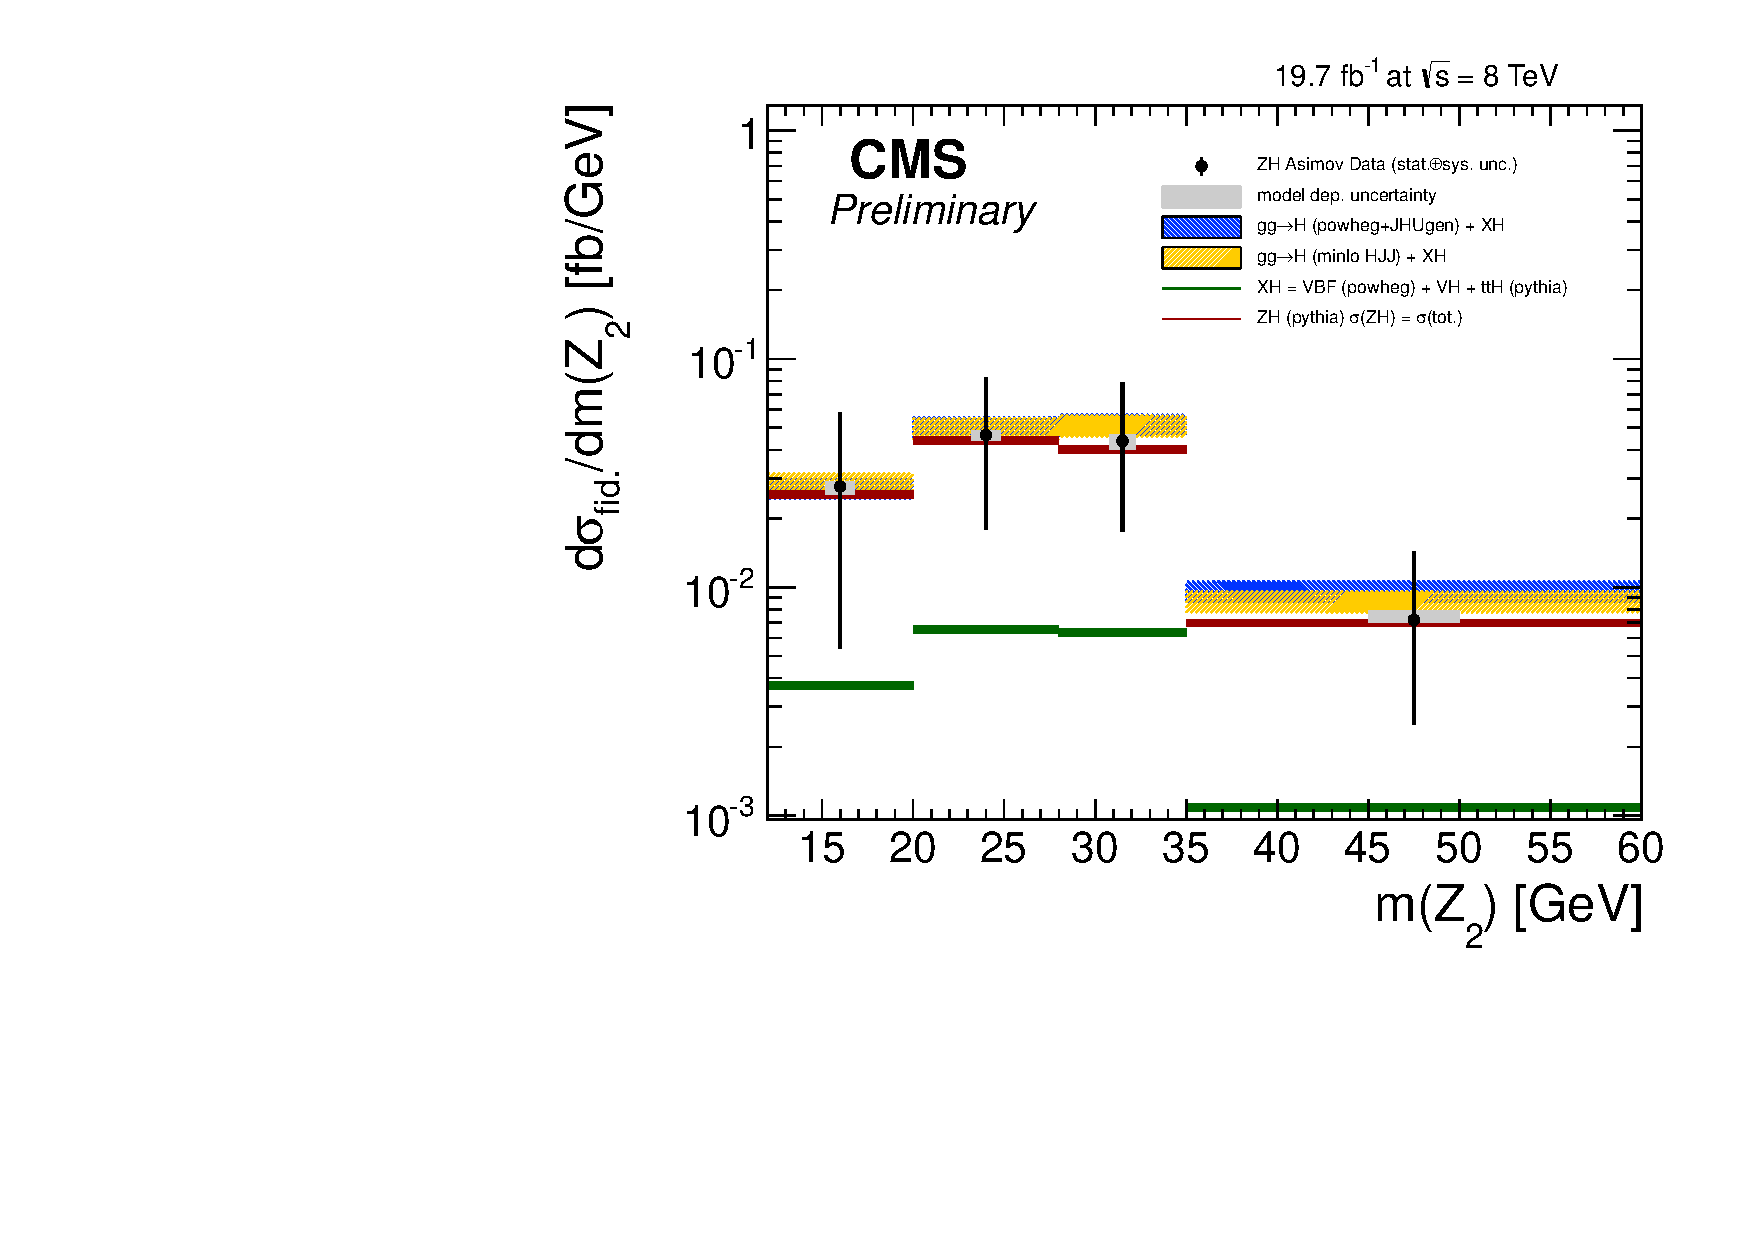
\includegraphics[width=0.48\textwidth,angle=0]{Plots/massZ2_unfoldwith_SM_125_logscale_ZHasimov.pdf}
      \label{fig:differential-results-ZHasimov:b}
    } \\
    \subfigure[$|y(\mathrm{H})|$]{
      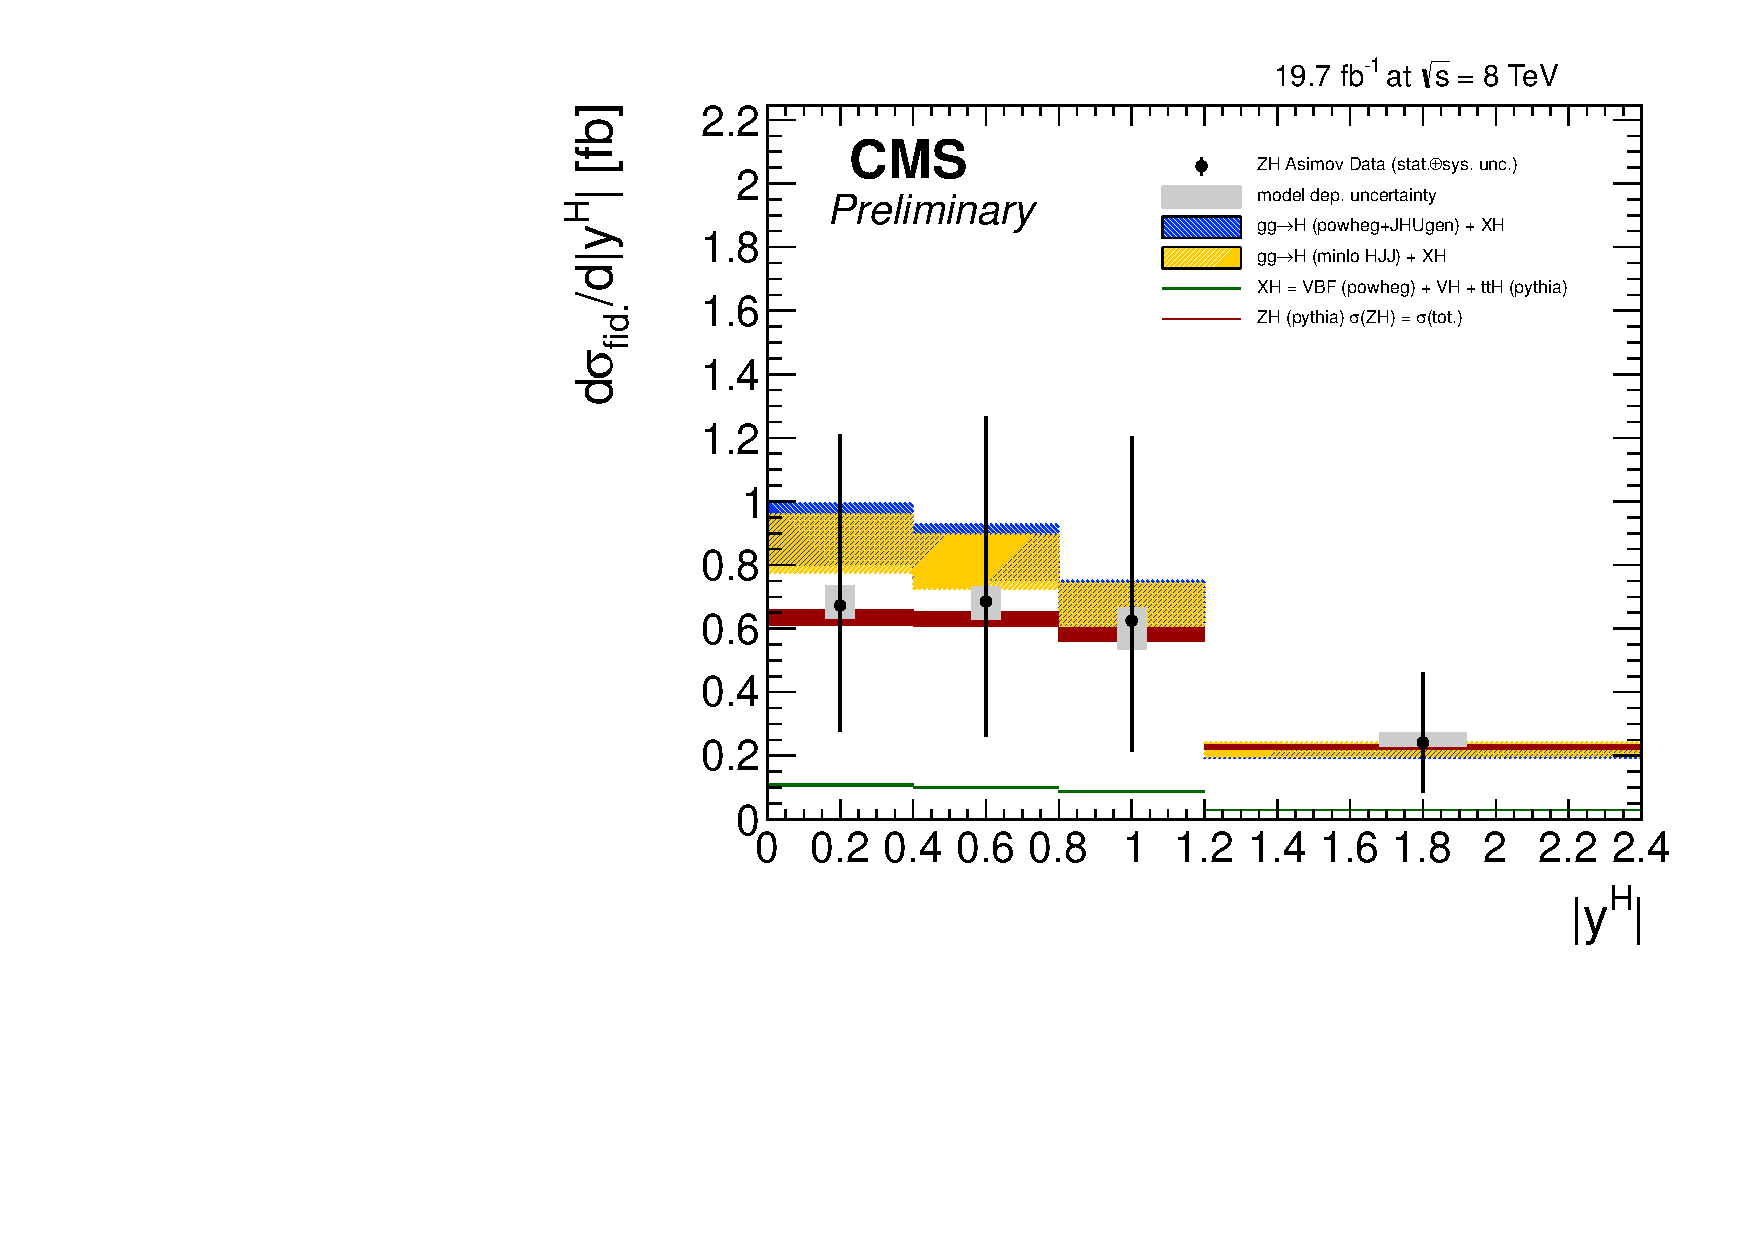
\includegraphics[width=0.48\textwidth,angle=0]{Plots/rapidity4l_unfoldwith_SM_125_ZHasimov.pdf}
      \label{fig:differential-results-ZHasimov:b}
    }
    \subfigure[$|\cos \theta^{*}|$]{
      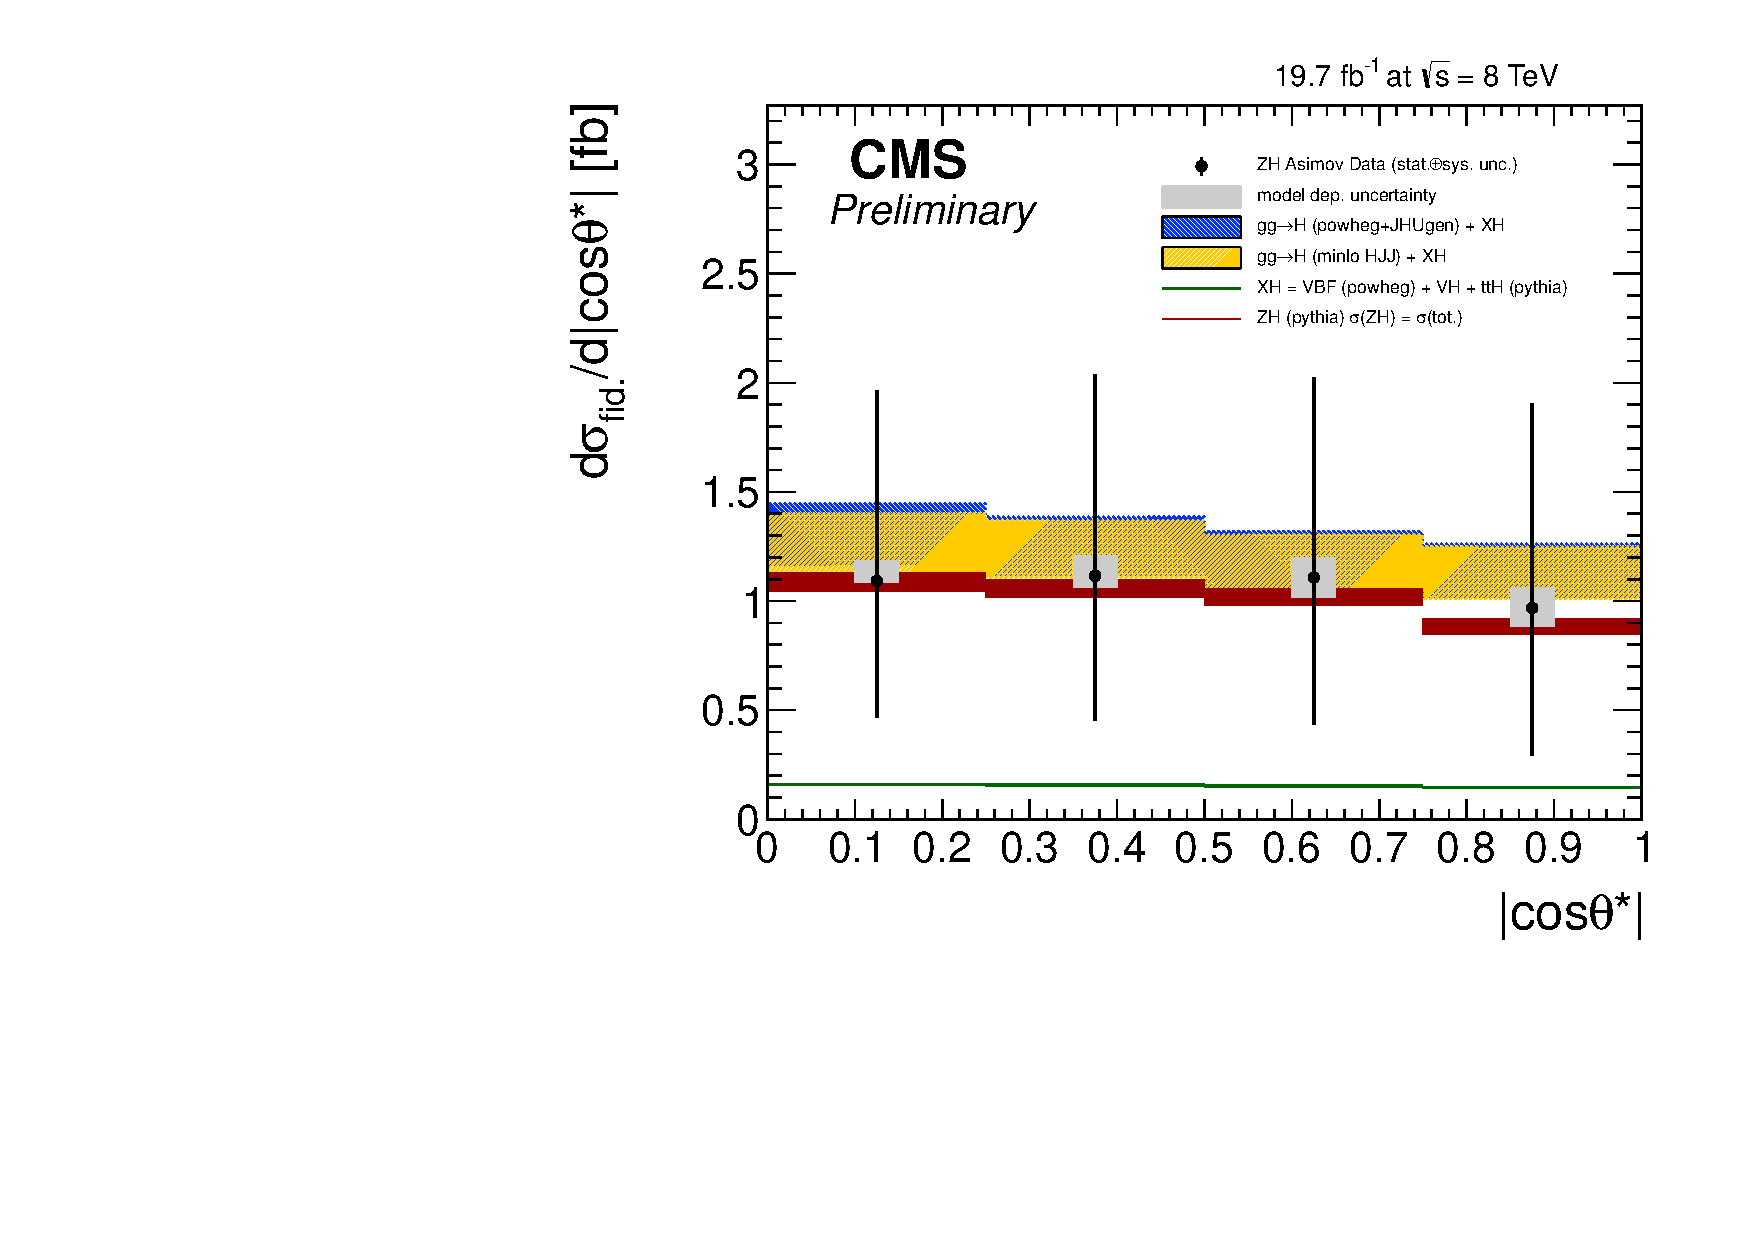
\includegraphics[width=0.48\textwidth,angle=0]{Plots/cosThetaStar_unfoldwith_SM_125_ZHasimov.pdf}
      \label{fig:differential-results-ZHasimov:c}
    } \\
    \subfigure[N(jets)]{
      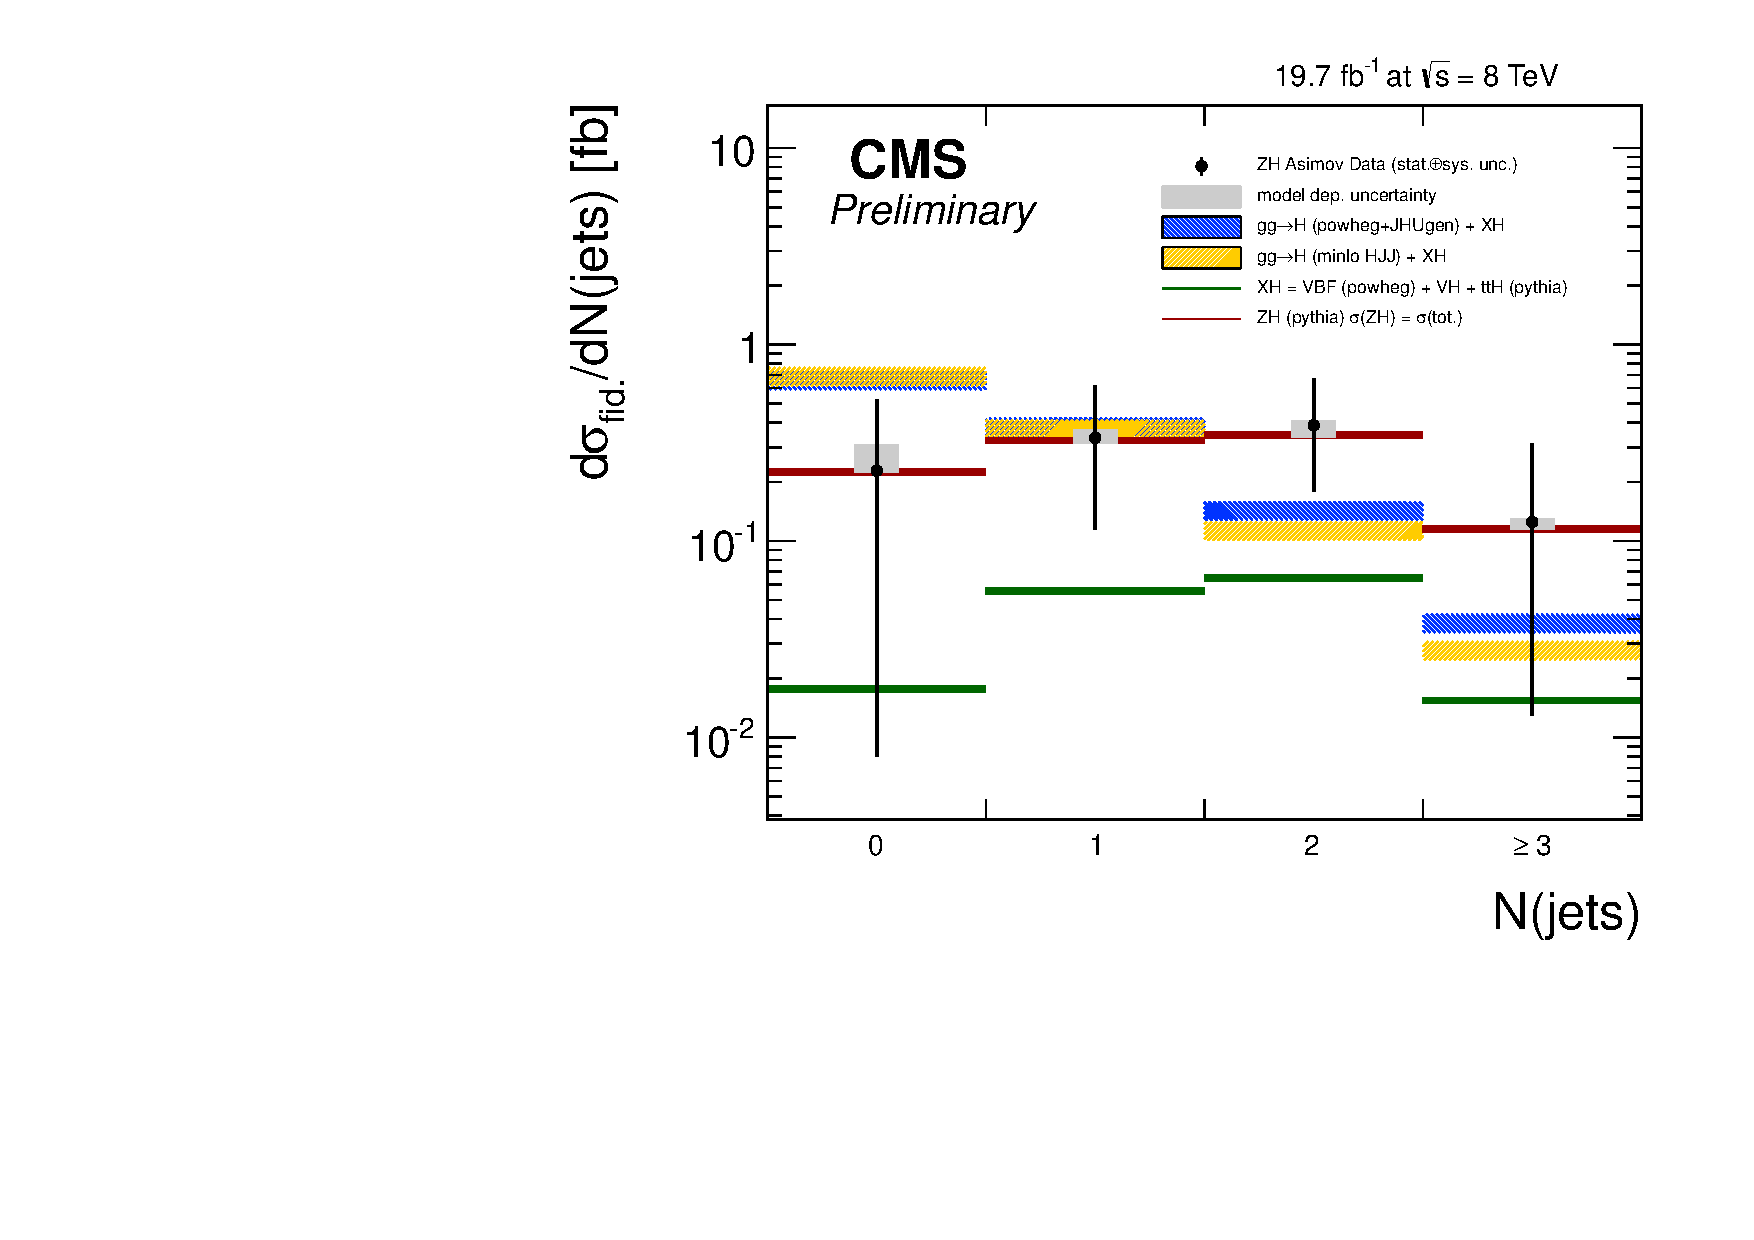
\includegraphics[width=0.48\textwidth,angle=0]{Plots/njets_reco_pt30_eta4p7_unfoldwith_SM_125_logscale_ZHasimov.pdf}
      \label{fig:differential-results-ZHasimov:d}
    }
    \caption{Results of the differential cross section measurement for different observables when the asimov dataset is generated assuming pure ZH production with cross section equal to the total SM cross section. The prediction for this pure ZH model is shown in red. The central value of the measurement is obtained using SM efficiencies with the gg$\rightarrow$H prediction from {\sc powheg+JHUgen} with m(H)= 125 $\GeV$, and the error bar represents the combined statistical and systematic uncertainty. The grey box represents the additional uncertainty incurred when using different models to unfold the observed data distribution back to particle level.
  }
  \label{fig:differential-results-restrictive_md}
 \end{center}
\end{figure}
